\section{Tidsplan}
For at tilrettelægge tiden, så alle dele af projektet nås inden projektet skal afleveres, er der lavet et Gantt-diagram. 
Når én farve slutter forventes det, at der stadig kan være en eventuel opsamling på arbejdsopgaven i buffer-ugen, samt hvis der er tid i de efterfølgende uger. 

Ud over Gantt-diagrammet laves der ugeplaner i starten af hver uge, så Gantt-diagrammets tidsplan kan følges og nås igennem projektperioden.
 
\begin{figure}[H]
\centering
\makebox[\textwidth][c]{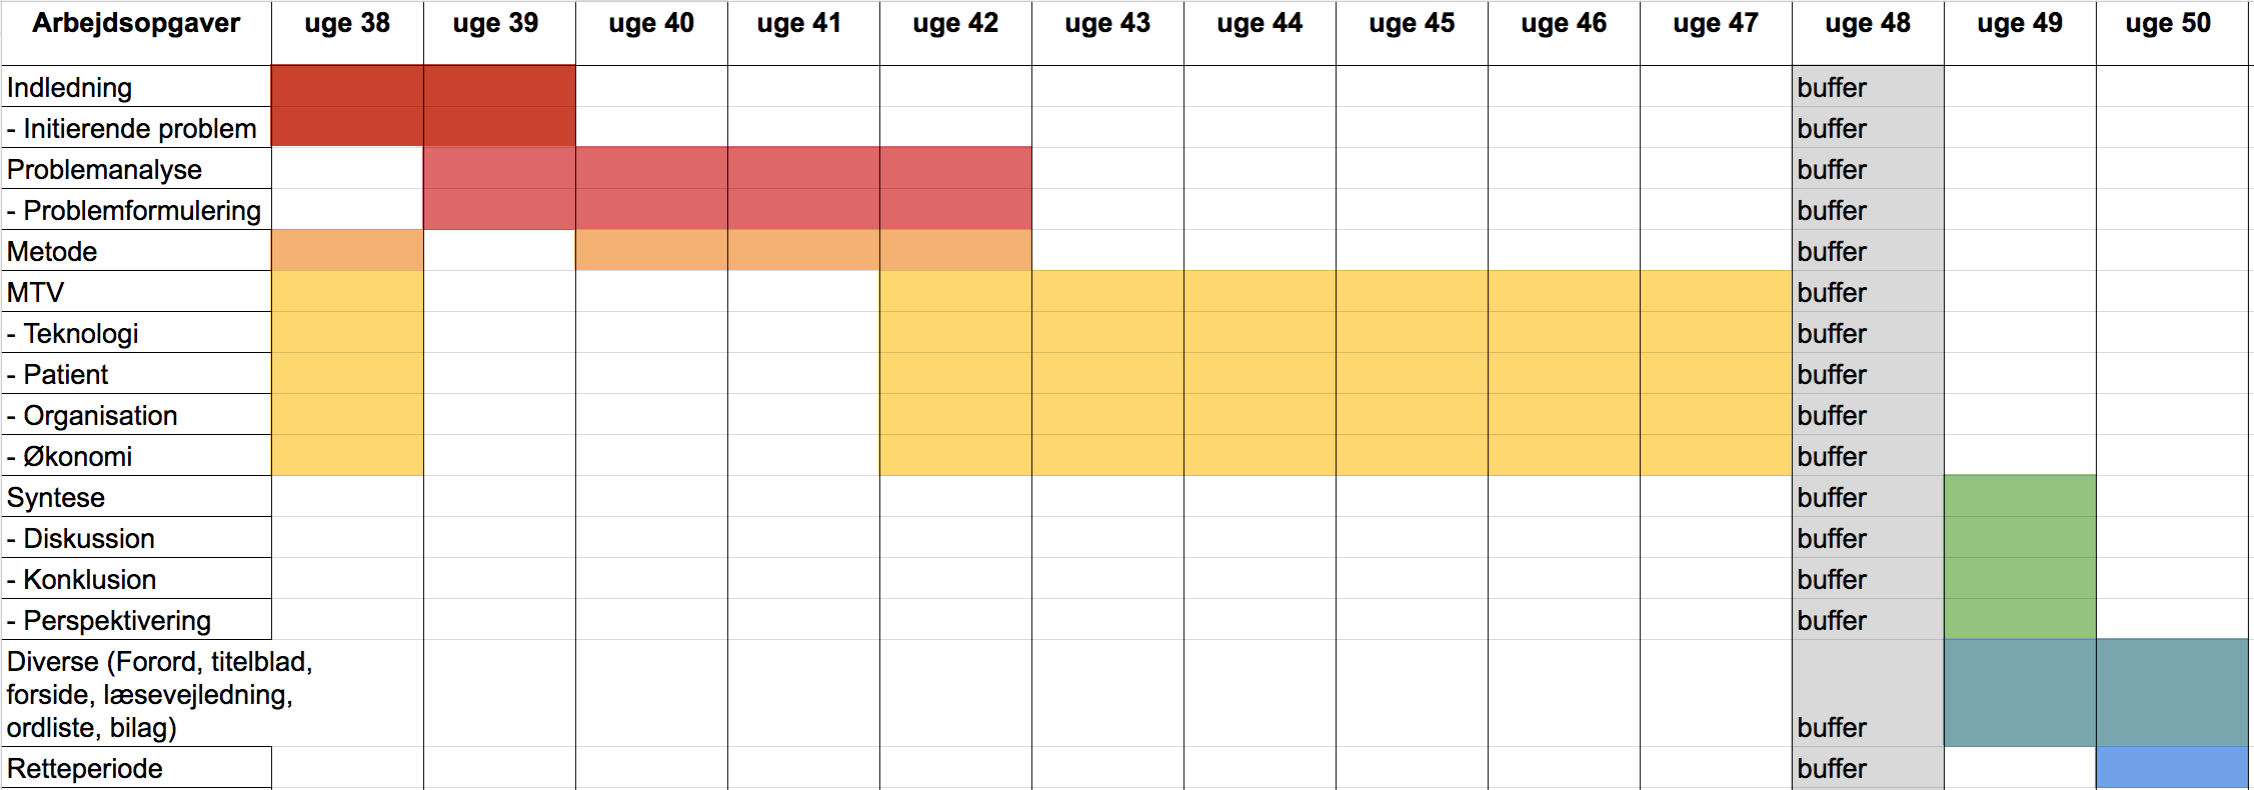
\includegraphics[width=1.2\textwidth]{Gantt}}
\caption{Gantt-diagram over, hvordan projektperioden er planlagt til at forløbe.}
\label{fig:tidsplan}
\end{figure}